\documentclass[11pt]{report}
\usepackage{amsmath, bm, xcolor, graphicx, listings}
\usepackage{courier} %for listings
\usepackage{caption}
\usepackage{subcaption}
\lstset{basicstyle=\footnotesize\ttfamily,breaklines=true} %listing font settings
%\lstset{framextopmargin=50pt} %listing font settings
\usepackage[english]{babel}
\setlength\parindent{0pt} %remove indentation in new paragraphs


\begin{document}
\title{\textbf{Poisson Solver (2D)}}
\author{Nikos Tryfonidis}
\date{2015}

\maketitle

\begin{abstract}
The current report summarizes the structure, use and results of a two-dimensional Poisson solver, 
created for the purpose of being integrated into a 2D Particle-In-Cell (PIC) code. After a brief introduction 
regarding the numerical solution of the 2D Poisson PDE in chapter 1, the structure of the code will be 
described in chapter 2. Verification of the code will be given in chapter 3, through a number of test cases. 
The different iterative methods that have been implemented are discussed in chapter 4, along with a brief review of their performance. Finally, the parallel implementation of the iterative solvers, using OpenMP threads, will be described in the fifth chapter, with a scaling performance review for each method.
\end{abstract}

\tableofcontents

\chapter{2D Poisson Equation: Numerical Solution}
The Poisson Equation and the associated boundary conditions form what is generally known as a 
\emph{Poisson Problem}: 

\begin{equation}
\nabla ^2 u = u_{xx} + u_{yy} = f(x,y)
\end{equation}

The Poisson Problem is one of the most well-known Elliptic Partial Differential Equations (PDE). A brief description of the numerical method followed in the code will be given here. Detailed analysis of the Poisson PDE and other methods can be found in most numerical analysis textbooks (for example \cite{leveque}).

\section{The Finite Difference Scheme}
The 5-point stencil discretization scheme is followed. A uniform Cartesian grid is used, where each point $x_i, y_j$ describes a point in 2D space, with $x_i = i\Delta x$ and $y_j = j\Delta y$. We assume that $0 \leq x \leq 1$ and $0 \leq y \leq 1$ for simplicity. Replacing the derivatives $u_{xx}$ and $u_{yy}$ in (1.1) with centered finite difference schemes, we end up with the following discretization scheme:

\begin{equation}
\frac{1}{(\Delta x)^2}(u_{i-1,j} -2u_{i,j} + u_{i+1,j}) + 
\frac{1}{(\Delta y)^2}(u_{i,j-1} -2u_{i,j} + u_{i,j+1}) = f_{i,j}
\end{equation}

Assuming that $\Delta x = \Delta y = h$, we get the simple finite difference scheme

\begin{equation}
u_{i-1,j} + u_{i+1,j} + u_{i,j-1} + u_{i,j+1} - 4u_{i,j} = h^2 f_{i,j}
\end{equation}

For a grid of $N \times N$ points in total, this scheme gives a linear system of $(N-2) \times (N-2)$ equations for the $(N-2) \times (N-2)$ unknowns (the excluded values are the boundaries, which are considered known). As an example to illustrate the system of equations, suppose we have a $5 \times 5$ grid of points, including boundaries, that represent our 2D space. 

\begin{figure}[h]
\centering
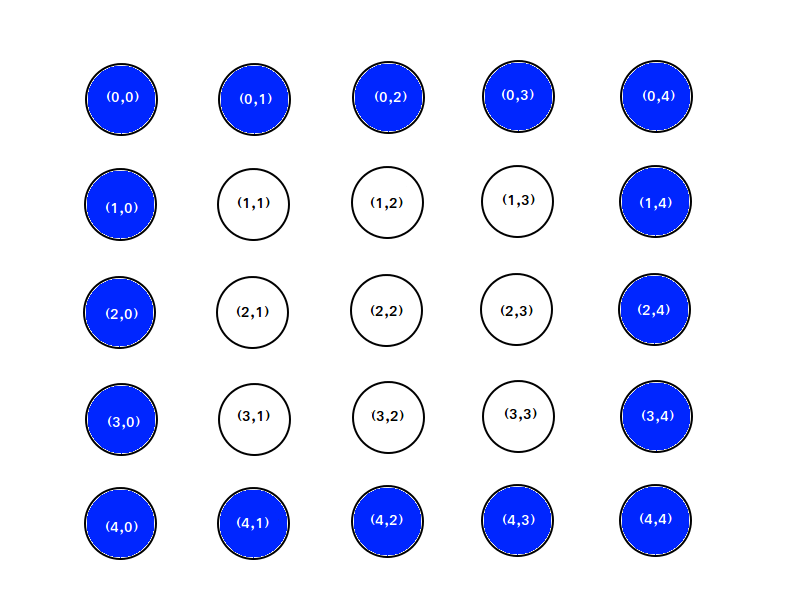
\includegraphics[scale=0.35]{images/grid}
\caption{A $5 \times 5$ two-dimensional grid. 
Boundary points, for which the solution is known, are shown in blue. }
\label{fig:Space grid 5x5}
\end{figure}

Applying the finite difference scheme (1.3) to each inner grid point $u_{i,j}$ leads us to a system of $(5-2) \times (5-2) = 9$ equations:

\begin{subequations}
\begin{align}
\bm{u_{1,1}}: 
\quad  & \textcolor{blue}{u_{0,1}} + u_{2,1} + \textcolor{blue}{u_{1,0}} + u_{1,2} - 4u_{1,1} = h^2 f_{1,1} \\
\bm{u_{1,2}}: 
\quad  & \textcolor{blue}{u_{0,2}} + u_{2,2} + u_{1,1} + u_{1,3} - 4u_{1,2} = h^2 f_{1,2} \\
\bm{u_{1,3}}: 
\quad  & \textcolor{blue}{u_{0,3}} + u_{2,3} + u_{1,2} + \textcolor{blue}{u_{1,4}} - 4u_{1,3} = h^2 f_{1,3} \\
\bm{u_{2,1}}: 
\quad  & u_{1,1} + u_{3,1} + \textcolor{blue}{u_{2,0}} + u_{2,2} - 4u_{2,1} = h^2 f_{2,1} \\
\bm{u_{2,2}}:
\quad  & u_{1,2} + u_{3,2} + u_{2,1} + u_{2,3} - 4u_{2,2} = h^2 f_{2,2} \\
\bm{u_{2,3}}: 
\quad  & u_{1,3} + u_{3,3} + u_{2,2} + \textcolor{blue}{u_{2,4}} - 4u_{2,3} = h^2 f_{2,3} \\
\bm{u_{3,1}}: 
\quad  & u_{2,1} + \textcolor{blue}{u_{4,1}} + \textcolor{blue}{u_{3,0}} + u_{3,2} - 4u_{3,1} = h^2 f_{3,1} \\
\bm{u_{3,2}}: 
\quad  & u_{2,2} + \textcolor{blue}{u_{4,2}} + u_{3,1} + u_{3,3} - 4u_{3,2} = h^2 f_{3,2} \\
\bm{u_{3,3}}: 
\quad  & u_{2,3} + \textcolor{blue}{u_{4,3}} + u_{3,2} + \textcolor{blue}{u_{3,4}} - 4u_{3,3} = h^2 f_{3,3}
\end{align}
\end{subequations}

\vspace{0.3cm}
We have arranged the equations row-wise, grouping elements with the same row number ($i$ index) together. We 
also see the boundary grid points in blue. These are considered to be known from the given boundary conditions.
\newline

We can now present the linear system of equations in matrix form,

\begin{equation}
\overleftrightarrow{\textbf{A}} \cdot \overrightarrow{\textbf{u}} = \overrightarrow{\textbf{b}},
\end{equation}

\vspace{0.3cm}

where $\overleftrightarrow{\textbf{A}}$ is the matrix equation, $\overrightarrow{\textbf{u}}$ is the vector of unknowns and $\overrightarrow{\textbf{b}}$ is the right-hand-side of the system of equations. Note that we will move the known boundary grid points to the right-hand-side of the matrix equation (again, shown in blue). The resulting matrix equation is

%%%Matrix with labels (uses parentheses): 
\begin{equation*}
\let\quad\thinspace
\bordermatrix{\text{}& \bm{u_{1,1}} & \bm{u_{1,2}} & \bm{u_{1,3}} & \bm{u_{2,1}} & \bm{u_{2,2}} & \bm{u_{2,3}} & \bm{u_{3,1}} & \bm{u_{3,2}} & \bm{u_{3,3}} \cr
   & -4 & 1 & 0 & 1 & 0 & 0 & 0 & 0 & 0  \cr
   & 1 & -4 & 1 & 0 & 1 & 0 & 0 & 0 & 0  \cr
   & 0 & 1 & -4 & 0 & 0 & 1 & 0 & 0 & 0  \cr 
   & 1 & 0 & 0 & -4 & 1 & 0 & 1 & 0 & 0  \cr
   & 0 & 1 & 0 & 1 & -4 & 1 & 0 & 1 & 0  \cr
   & 0 & 0 & 1 & 0 & 1 & -4 & 0 & 0 & 1  \cr
   & 0 & 0 & 0 & 1 & 0 & 0 & -4 & 1 & 0  \cr
   & 0 & 0 & 0 & 0 & 1 & 0 & 1 & -4 & 1  \cr
   & 0 & 0 & 0 & 0 & 0 & 1 & 0 & 1 & -4 
    }
\cdot
\begin{pmatrix}
u_{1,1} \\ u_{1,2} \\ u_{1,3} \\ u_{2,1} \\ u_{2,2} \\ u_{2,3} \\ u_{3,1} \\ u_{3,2} \\ u_{3,3}
\end{pmatrix}
=
\begin{pmatrix}
h^2f_{1,1} + \textcolor{blue}{u_{0,1}} + \textcolor{blue}{u_{1,0}} \\ 
h^2f_{1,2} + \textcolor{blue}{u_{0,2}} \\ 
h^2f_{1,3} + \textcolor{blue}{u_{0,3}} + \textcolor{blue}{u_{1,4}} \\
h^2f_{2,1} + \textcolor{blue}{u_{2,0}} \\
h^2f_{2,2} \\
h^2f_{2,3} + \textcolor{blue}{u_{2,4}} \\
h^2f_{3,1} + \textcolor{blue}{u_{4,1}} + \textcolor{blue}{u_{3,0}} \\
h^2f_{3,2} + \textcolor{blue}{u_{3,2}} + \textcolor{blue}{u_{4,2}} \\
h^2f_{3,3} + \textcolor{blue}{u_{4,3}} + \textcolor{blue}{u_{3,4}}
\end{pmatrix}
\end{equation*}
\vspace{0.75cm}

We see that the resulting $\overleftrightarrow{\textbf{A}}$ matrix is block-tridiagonal:

\begin{equation}
\overleftrightarrow{\textbf{A}} = 
\begin{pmatrix}
\bm{T} & \bm{I} & \bm{0} \\
\bm{I} & \bm{T} & \bm{I} \\
\bm{0} & \bm{I} & \bm{T}
\end{pmatrix}
\end{equation}
\vspace{0.5cm}
\begin{equation}
\bm{T} =
\begin{pmatrix}
-4 & 1 & 0 \\
1 & -4 & 0 \\
0 & 1 & -4
\end{pmatrix}
, \quad
\bm{I} =
\begin{pmatrix}
1 & 0 & 0 \\
0 & 1 & 0 \\
0 & 0 & 1
\end{pmatrix}
, \quad
\bm{0} =
\begin{pmatrix}
0 & 0 & 0 \\
0 & 0 & 0 \\
0 & 0 & 0
\end{pmatrix}
\end{equation}

\vspace{0.5cm}

This linear system of equations can be solved with a variety of methods (direct, iterative etc). Our focus will be on iterative methods.

\section{Error and Stability}
We will not go into the details of error and stability analysis in this report, since these are well-known 
and can be found in most relevant texts (e.g. \cite{leveque}). We should simply keep in mind that the local truncation error of the 5-point stencil finite difference scheme we are using is $O(h^2)$ and that the method is stable, so the global error of the method is also $O(h^2)$. In case we do not assume $\Delta x = \Delta y = h$, this 
simply means that the error is $O\left( (\Delta x)^2, (\Delta y)^2 \right)$.

\chapter{The Code}
In this chapter, the structure and use of the code will be described. The project has been arranged into 
separate directories. The source code is in "src", with corresponding header files in "headers", one for each 
.c source file (other than "main.c"). Object files (".o") are automatically placed into the "obj" directory by the makefile. Output files are also placed into the "output" directory. The python visualization script used 
for plotting the output is also in "output". Finally, "documentation" contains the current report.

In the following sections, we will briefly go through instructions on how to use the code, and we will review its structure.

\section{Compilation and Execution}
The code does not contain any external libraries and should compile without problems on any linux system with a C compiler. To compile, go to the central directory of the project, where the makefile is located, and type "make". This will create the executable file in the same directory, with object files in "obj". To delete the executable and the object files, type "make clean".

To run, simply run the executable from the command line, giving two arguments (number of grid points in dimensions X and Y, respectively). For example, the following will run the program with 101 grid points in X and Y:

\begin{lstlisting}
./poisson2D 101 101
\end{lstlisting}

\section{Code Structure}
Here we will briefly go through the code structure, by explaining the work done by each of the source files. 

\begin{description}
  \item[main.c] The main file simply wraps all pieces of the program together and can be seen as a program outline. First it reads the command line arguments and it allocates the required memory. Then, it sets up the problem, by setting the appropriate Boundary Conditions and right-hand-side function f(x,y) (see "setup.c").
  \item[io.c] Contains functions that read command line arguments and write file output.
  \item[setup.c] Contains functions that set boundary conditions and the right-hand-side function. This is where the user can specify the Poisson problem he/she wants to solve. \emph{Boundary conditions} can be set for each one of the four boundaries separately, by the $"setBoundaries2D"$ function. The RHS function is set by $"setRHS2D"$.
  \item[memory.c] Contains the $"array2D_contiguous"$ function, that dynamically allocates a two-dimensional array of doubles, contiguous in memory. Also contains the $"free_array2D_contiguous"$ function, that frees memory allocated by the previous function.
  \item[poisson2D.c] The solver function. It iterates the solution for the appropriate number of iterations, until the desired accuracy is reached (or a maximum number of iterations is done). The iteration method of choice is passed into the function as an argument (function pointer). Error tolerance, maximum iterations, iterations per residual check are all set in this function. Also contains the residual calculation function.
  \item[iterative.c] Contains the different iterative methods that may be used, and that are called by $"solvePoisson2D"$. Currently, the Jacobi, Gauss-Seidel and Successive Overrelaxation methods have been implemented.
\end{description}

The space dimensions $(x_0, x_L), (y_0, y_L)$ are set in \emph{definitions.h}, inside the \emph{headers} directory.

\section{Data Structures}
The main data structure used is a two-dimensional array of doubles, that represents the discretized space grid. The dimensions of the grid are given from the command line arguments the user provides. Memory for the 2D array is allocated by the $"array2D_contiguous"$ function in \emph{memory.c}.
\newline

Also, another two-dimensional array of the same dimensions is the right-hand-side function (RHS) of the Poisson Equation, $f(x,y)$. Memory for the RHS function is allocated in the same way as for the grid. The values of RHS for each grid point is set by the $"setRHS2D"$ function in \emph{setup.c}.

\section{Solving a Poisson Problem}
To solve a given Poisson problem, the user must perform the following actions:

\begin{enumerate}
  \item Set Boundary Conditions in \emph{setBoundaries2D} (setup.c).
  \item Set the RHS function of the Poisson problem in \emph{setRHS2D} (setup.c).
  \item Choose the desired iterative method in main function (main.c).
  \item Compile the program by typing "make" in the main directory (where the makefile is located).
  \item Run the executable with the desired number of grid points in each of the two dimensions.
\end{enumerate}

\section{Output}
Output is written in the "output" directory. Two output files are written:

\begin{description}
  \item[output.txt] Contains the 2D solution grid.
  \item[gridData.txt] Contains grid data $\left( (x_0, x_L), (y_0, y_L) \right) $, step sizes ($dx, dy$) and number of grid points in each dimension ($N_x, N_y$). Data from this file is read by the visualization python script in the same folder, in order to create a plot of the results.
\end{description}

The solution is visualized by the python script \emph{visualize.py}, in the output directory.
The script requires \emph{numpy} and \emph{matplotlib}, two well-known packages for scientific computing in Python.

These can be easily installed in any Linux system, for example in Ubuntu:

\begin{lstlisting}
sudo apt-get install python-numpy python-matplotlib
\end{lstlisting}

This python script reads grid meta-data from \emph{gridData.txt} and the solution from \emph{output.txt} and creates a 3D plot of the solution.

To create the plot, the user must simply run the script by typing:

\begin{lstlisting}
python visualize.py
\end{lstlisting}

\chapter{Verification}
In this chapter we will verify the correctness of the 2D Poisson solver, through three basic examples that have known analytic solutions. By comparing the numerical solution with the analytic one, we will show that the solver produces correct results.
\newline

Each example has detailed instructions on how to set up the Poisson problem studied, so the following sections can also be used as examples on how to use the code. The \emph{Gauss-Seidel} iterative method was chosen for these examples, with a tolerance of $\Delta x^2$ for the residual check.
\newline

For the following examples, the domain was chosen to be $0 \leq x,y \leq 1$, which is set in \emph{headers/definitions.h} as follows:

\begin{lstlisting}
#define X0 0.0
#define XL 1.0
#define Y0 0.0
#define YL 1.0
\end{lstlisting}

We also used 101 grid points for each dimension, dividing each dimension into $(101 - 1)$ pieces, so that 
\begin{equation}
\Delta x = \Delta y = (Length) / (101 - 1) = 1.0 / 100 = 0.01
\end{equation}
\newpage

\section{Zero RHS (Laplace Equation)}
In this problem, we will solve a Poisson problem with no right-hand-side function. Let us assume that the (known) solution $u(x,y)$ is 

\begin{equation}
u(x,y) = 3x + 4y
\end{equation}

The corresponding Poisson problem is then

\begin{subequations}
\begin{align}
\nabla ^2 u = &u_{xx} + u_{yy} = 0 \\
u(x,0) = 3x \quad \quad \quad & \quad \quad \quad u(x,y_L) = 3x + 4y_L \\
u(0,y) = 4y \quad \quad \quad & \quad \quad \quad u(x_L,y) = 3x_L + 4y
\end{align}
\end{subequations}

Equation $(3.2a)$, along with boundary conditions $(3.2b)$ and $(3.2c)$ are also known as a Laplace problem, a special case of the Poisson problem with a zero right-hand-side function. We will now solve this Poisson problem and compare the numerical solution with the analytic $(3.1)$.

\subsection*{Setting Up The Problem}
As explained in paragraph \emph{2.4}, the functions that are used to set up the desired Poisson problem are in \emph{setup.c}. Boundary conditions are given by the known solution \emph{(3.1)}, while the RHS function is zero for this problem. 
\newline

We set the Boundary Conditions:

\begin{lstlisting}
double fBC(double x, double y) 
{
    return 3.0*x + 4.0*y;
}
\end{lstlisting}

and the RHS function:

\begin{lstlisting}
double f(double x, double y) 
{
    return 0.0;
}
\end{lstlisting}

\subsection*{Running the Solver}
After we set up the problem as shown, we compile the program and run. To specify 101 grid points for $x$ and $y$, we run the executable as follows:

\begin{lstlisting}
./poisson2D 101 101
\end{lstlisting}

Once the program has finished, output is ready in \emph{output/output.txt}. We can plot the solution by running the python script \emph{visualize.py}, which will create a 3D surface plot of our solution. In the next figure, the analytic and numerical solutions are shown side by side for comparison:

\begin{figure}[h!]
\centering
\begin{subfigure}{0.5\textwidth}
  \centering
  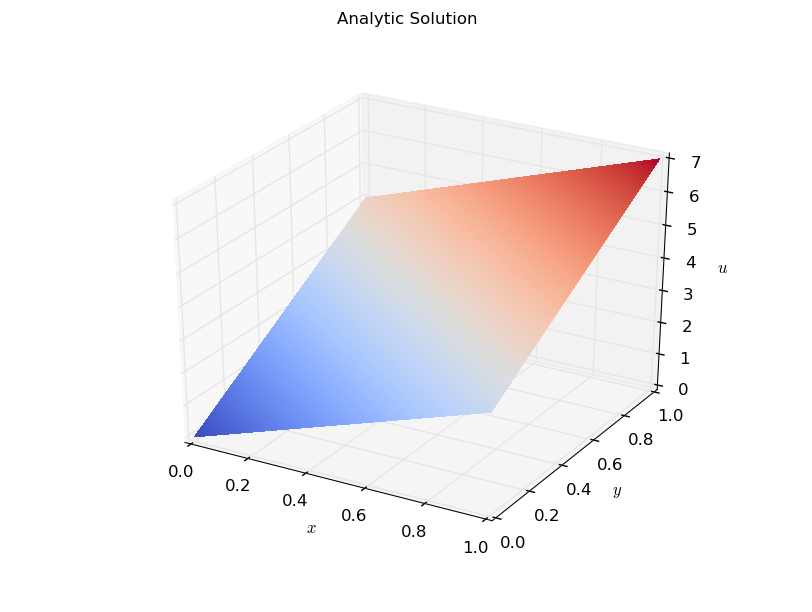
\includegraphics[width=1.0\linewidth]{images/example1_analytic}
  \caption{Analytic solution}
  \label{fig:sub1}
\end{subfigure}%
\begin{subfigure}{0.5\textwidth}
  \centering
  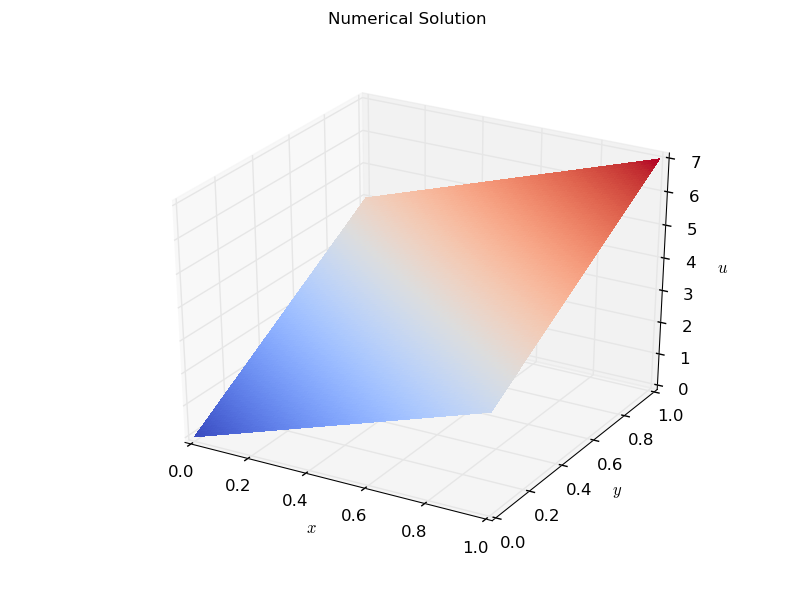
\includegraphics[width=1.0\linewidth]{images/example1_numerical}
  \caption{Numerical solution}
  \label{fig:sub2}
\end{subfigure}
\begin{subfigure}{0.6\textwidth}
  \centering
  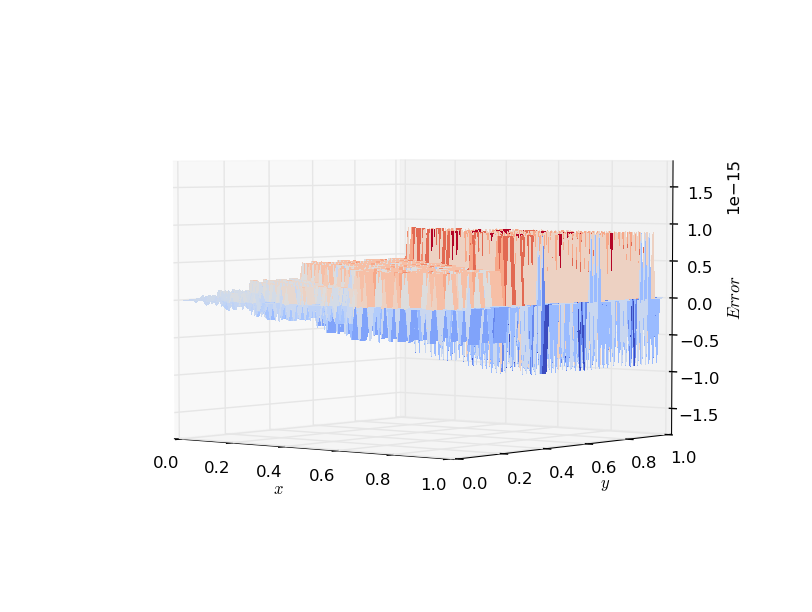
\includegraphics[width=1.0\linewidth]{images/example1_error}
  \caption{Error}
  \label{fig:sub2}
\end{subfigure}
\caption{Analytic (a) and numerical (b) solution for the current Poisson problem, with a surface plot of the  error in (c).}
\label{fig:example1}
\end{figure}

We see that the numerical solution is identical to the analytic one, and the error is shown to be of the order of $10^{-15}$ (machine precision, since with a constant right-hand-side we are effectively calculating averages). 

\section{Simple Linear RHS}
Now, we will solve a Poisson problem with a simple linear right-hand-side function. Let us assume that the (known) solution $u(x,y)$ is 

\begin{equation}
u(x,y) = x^2 + y^2
\end{equation}

The corresponding Poisson problem is now

\begin{subequations}
\begin{align}
\nabla ^2 u = &u_{xx} + u_{yy} = 2 + 2 = 4 \\
u(x,0) = x^2 \quad \quad \quad & \quad \quad \quad u(x,y_L) = x^2 + (y_L)^2 \\
u(0,y) = y^2 \quad \quad \quad & \quad \quad \quad u(x_L,y) = (x_L)^2 + y^2
\end{align}
\end{subequations}

We will now solve this Poisson problem and compare the numerical solution with the analytic $(3.4)$.

\subsection*{Setting Up The Problem}
We set up the desired Poisson problem, as shown in the previous example, in \emph{setup.c}. Boundary conditions are given by the known solution \emph{(3.4)}, while the RHS function is equal to $4$ for this problem. 
\newline

We set the Boundary Conditions:

\begin{lstlisting}
double fBC(double x, double y) 
{
    return x*x + y*y;
}
\end{lstlisting}

and the RHS function:

\begin{lstlisting}
double f(double x, double y) 
{
    return 4.0;
}
\end{lstlisting}

\subsection*{Running the Solver}
We compile and run, once again, with 101 grid points in each dimension, as before:
\newline 

\begin{lstlisting}
./poisson2D 101 101
\end{lstlisting}

We produce the surface plot of the results with \emph{visualize.py}. In the next figure, the analytic and numerical solutions are shown side by side for comparison:

\begin{figure}[h!]
\centering
\begin{subfigure}{0.5\textwidth}
  \centering
  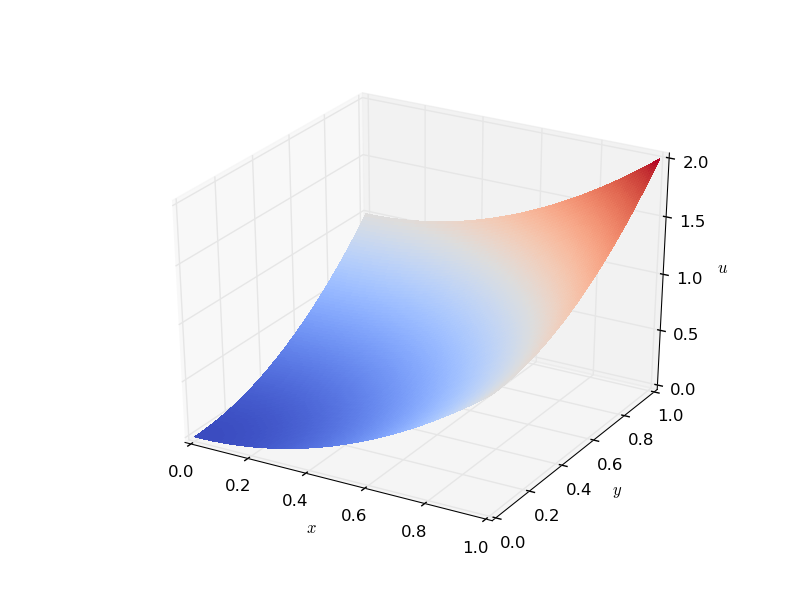
\includegraphics[width=1.0\linewidth]{images/example2_analytic}
  \caption{Analytic solution}
  \label{fig:sub2.1}
\end{subfigure}%
\begin{subfigure}{0.5\textwidth}
  \centering
  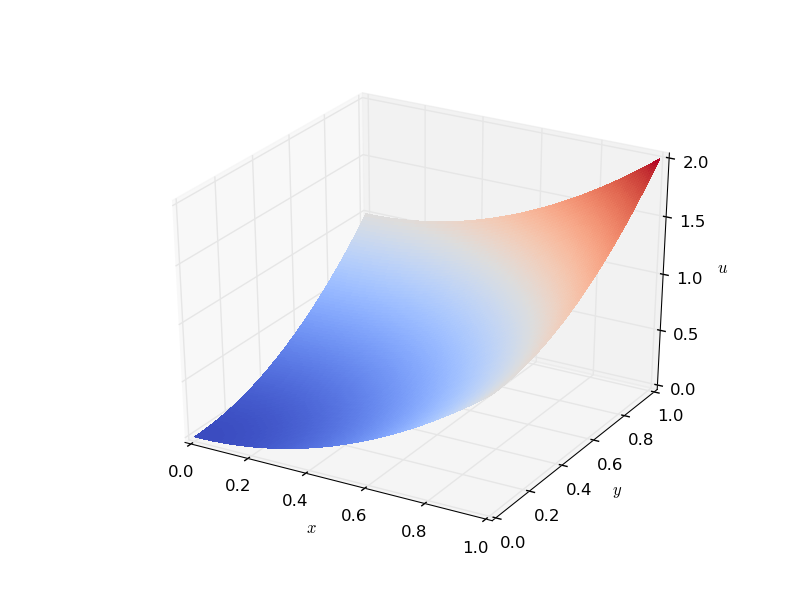
\includegraphics[width=1.0\linewidth]{images/example2_numerical}
  \caption{Numerical solution}
  \label{fig:sub2.2}
\end{subfigure}
\begin{subfigure}{0.6\textwidth}
  \centering
  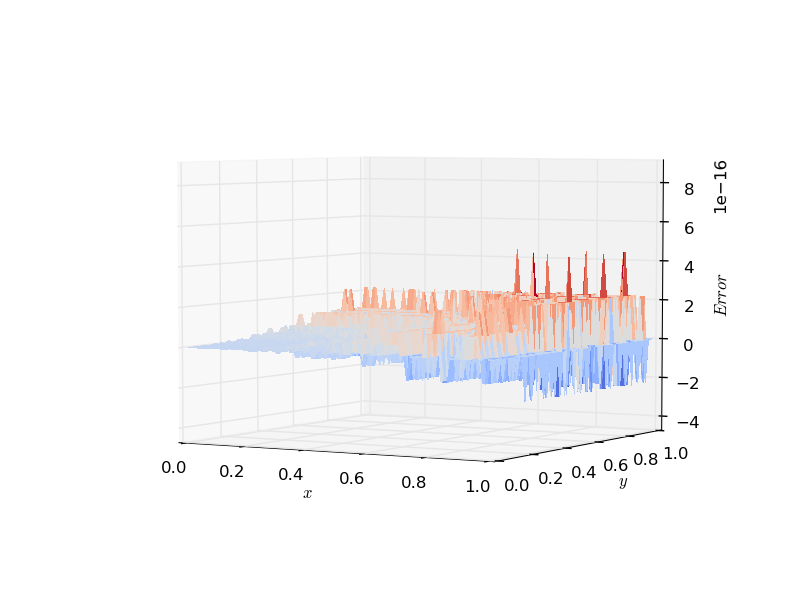
\includegraphics[width=1.0\linewidth]{images/example2_error}
  \caption{Error}
  \label{fig:sub2.3}
\end{subfigure}
\caption{Analytic (a) and numerical (b) solution for the current Poisson problem, with a surface plot of the  error in (c).}
\label{fig:example2}
\end{figure}

We see that the numerical solution is identical to the analytic one, and the error is shown to be of the order of $10^{-16}$ (machine precision again, since with a constant right-hand-side we are effectively calculating averages). 

\newpage
\section{Sinusoidal RHS}
Now, we will solve a Poisson problem with a slightly more complex right-hand-side function. Let us assume that the (known) solution $u(x,y)$ is 

\begin{equation}
u(x,y) = sin\left[ 2\pi \left( x + y\right) \right]
\end{equation}

The corresponding Poisson problem is now

\begin{subequations}
\begin{align}
\nabla ^2 u = u_{xx} + u_{yy} &= -8\pi^2 sin\left[ 2\pi \left( x + y\right) \right] \\
u(x,0) = sin\left[ 2\pi \left( x \right) \right] \quad \quad & \quad \quad 
u(x,y_L) = sin\left[ 2\pi \left( x + y_L\right) \right]\\
u(0,y) =  sin\left[ 2\pi \left( y \right) \right] \quad \quad & \quad \quad 
u(x_L,y) =  sin\left[ 2\pi \left( x_L + y\right) \right]
\end{align}
\end{subequations}

We will now solve this Poisson problem and compare the numerical solution with the analytic $(3.6)$.

\subsection*{Setting Up The Problem}
We set up the desired Poisson problem, as shown in the previous examples, in \emph{setup.c}. Boundary conditions are given by the known solution \emph{(3.6)}, while the RHS function is $f(x,y) =  -8\pi^2 sin\left[ 2\pi \left( x + y\right) \right]$ for this problem. 
\newline

We set the Boundary Conditions:

\begin{lstlisting}
double fBC(double x, double y) 
{
    return sin(2.0*M_PI*(x+y));
}
\end{lstlisting}

and the RHS function:

\begin{lstlisting}
double f(double x, double y) 
{
    return -8.0*M_PI*M_PI*sin(2.0*M_PI*(x+y));
}
\end{lstlisting}

\subsection*{Running the Solver}
We compile the program and run with 101 grid points in each dimension, as before:
\newline 

\begin{lstlisting}
./poisson2D 101 101
\end{lstlisting}

We produce the surface plot of the results with \emph{visualize.py}. In the next figure, the analytic and numerical solutions are shown side by side for comparison. Also, the error surface plot is shown; this was created by plotting the difference of the analytic minus the numerical solution.

\begin{figure}[h!]
\centering
\begin{subfigure}{0.5\textwidth}
  \centering
  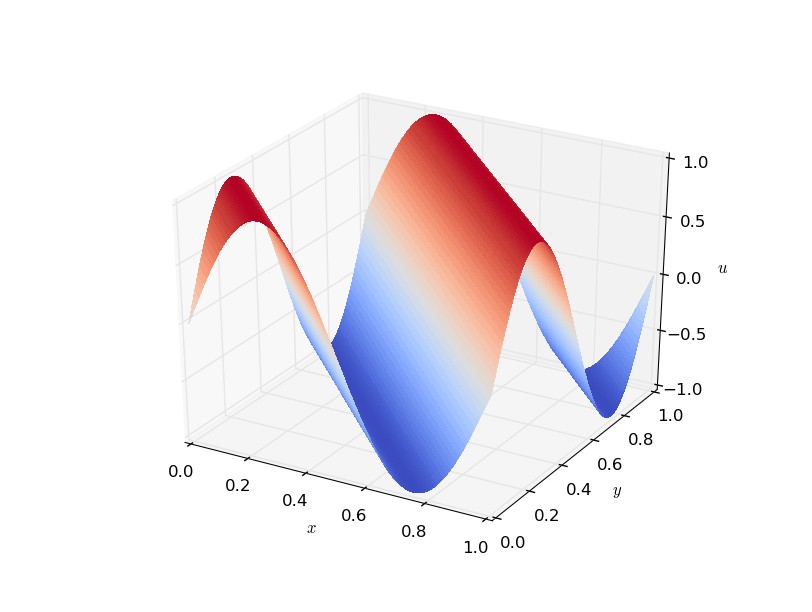
\includegraphics[width=1.0\linewidth]{images/example3_analytic}
  \caption{Analytic solution}
  \label{fig:sub3.1}
\end{subfigure}%
\begin{subfigure}{0.5\textwidth}
  \centering
  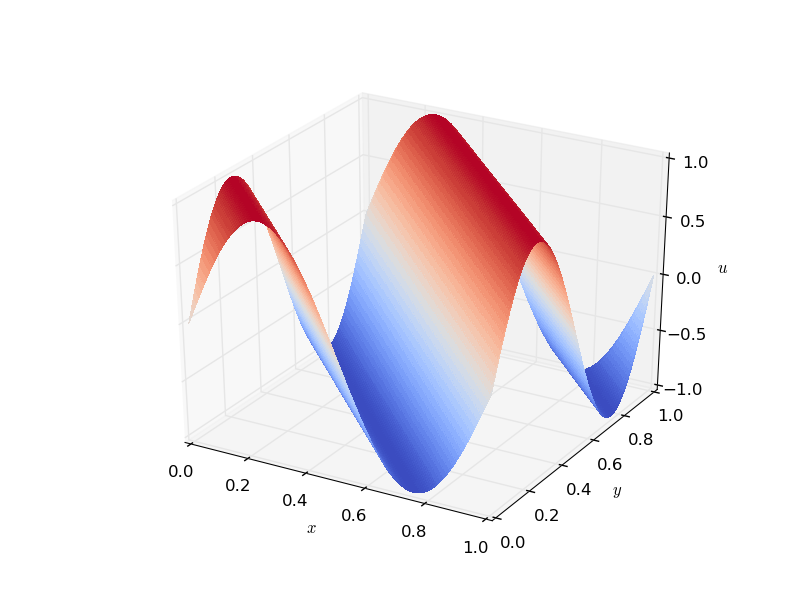
\includegraphics[width=1.0\linewidth]{images/example3_numerical}
  \caption{Numerical solution}
  \label{fig:sub3.2}
\end{subfigure}
\begin{subfigure}{0.6\textwidth}
  \centering
  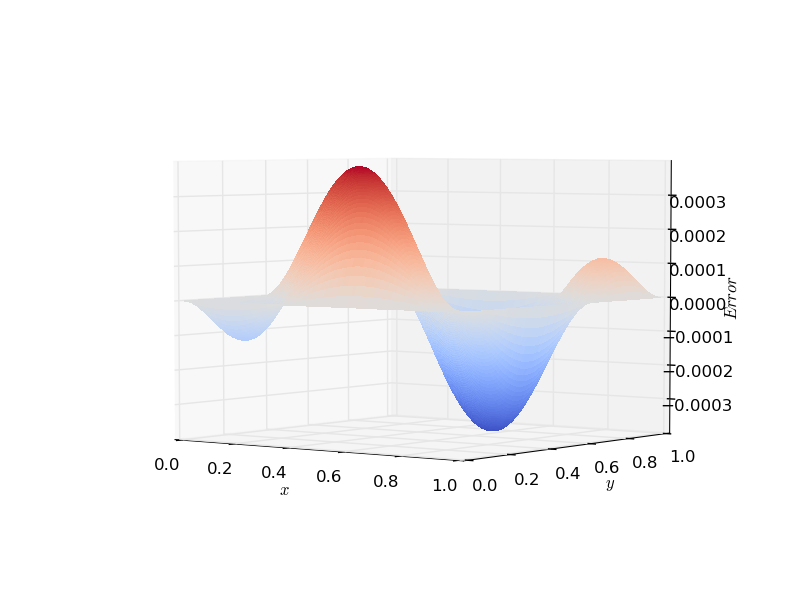
\includegraphics[width=1.0\linewidth]{images/example3_error}
  \caption{Error}
  \label{fig:sub3.3}
\end{subfigure}
\caption{Analytic (a) and numerical (b) solution for the current Poisson problem, with a surface plot of the  error in (c).}
\label{fig:example3}
\end{figure}

We see that the numerical solution is identical to the analytic one, and the error is shown to be, as expected, of the order of $O(h^2) = O(0.0001)$, where $h = \Delta x = \Delta y = 0.01$. 

\section{Minimizing the Error}
As a last verification test, we will show that our solution becomes better (i.e. the error becomes smaller), as we refine our grid. We will use the previous section's Poisson problem to show this.
\newline

We will plot the error, using an increasing number of grid points. We expect the error to get smaller as $dx, dy$ become smaller. The results are shown in the following two figures:

\begin{figure}[h!]
\centering
\begin{subfigure}{0.5\textwidth}
  \centering
  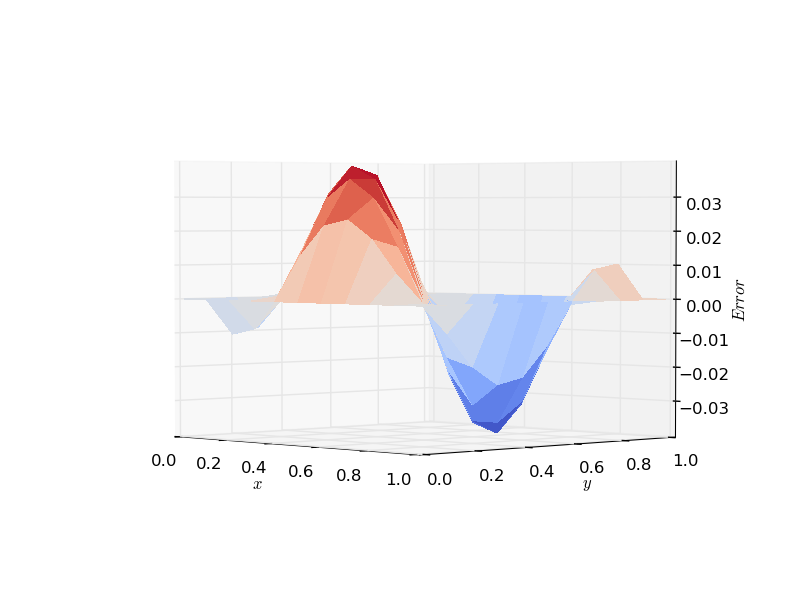
\includegraphics[width=1.0\linewidth]{images/example4_10}
  \caption{$N = 10 \quad (h = 0.1)$}
\end{subfigure}
\begin{subfigure}{0.5\textwidth}
  \centering
  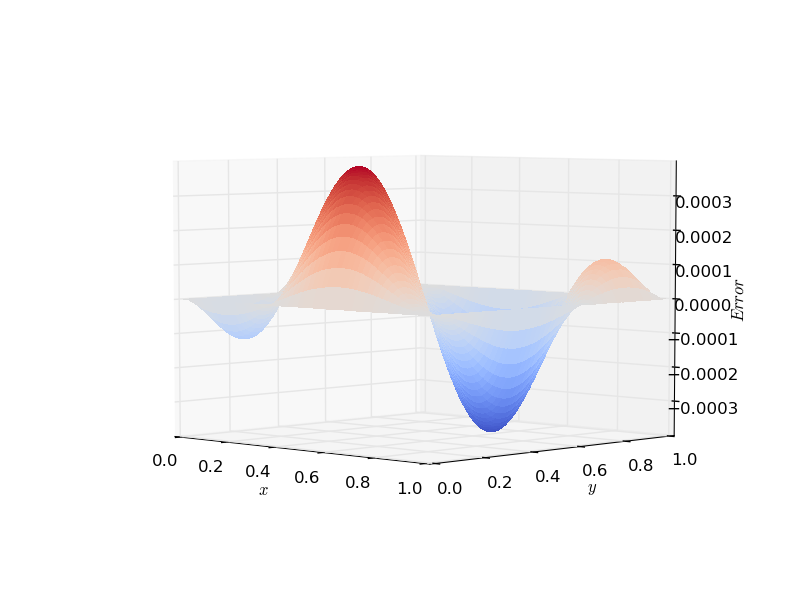
\includegraphics[width=1.0\linewidth]{images/example4_100}
  \caption{$N = 100  \quad (h = 0.01)$}
\end{subfigure}
\caption{Error ($u_{analytic} - u_{numerical}$) for decreasing $h = dx = dy$. The error gets smaller as we go from 10 to 100 grid points (see Error axis range).}
\label{fig:example4.1}
\end{figure}

We notice that the error does get smaller as $h$ decreases, and also it is of order $O(h^2)$, as expected. Even smaller $h$ choices are shown in the next figure:

\begin{figure}[h!]
\centering
\begin{subfigure}{0.5\textwidth}
  \centering
  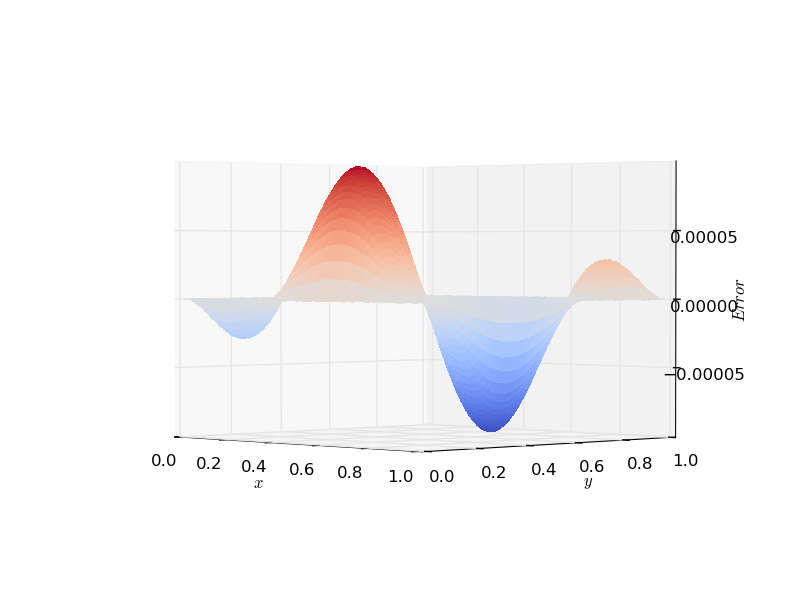
\includegraphics[width=1.0\linewidth]{images/example4_200}
  \caption{$N = 200 \quad (h = 0.005)$}
\end{subfigure}\\
\begin{subfigure}{0.5\textwidth}
  \centering
  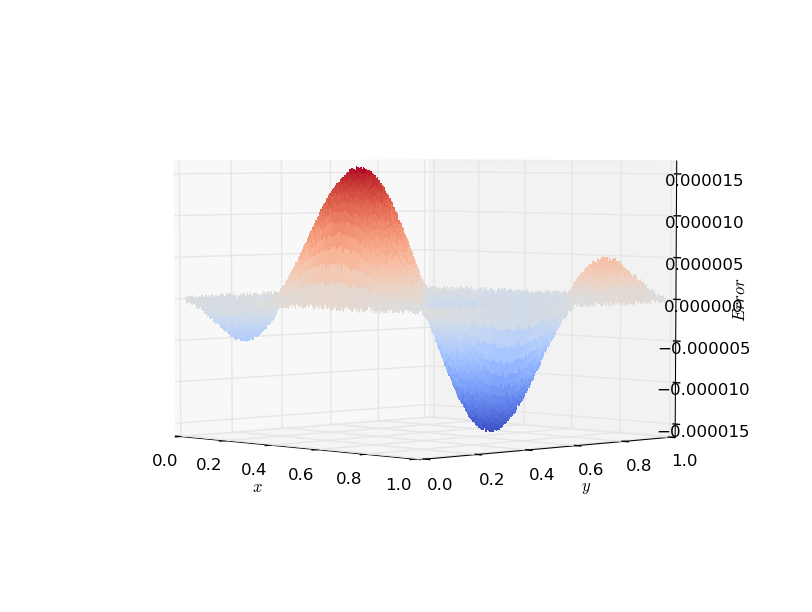
\includegraphics[width=1.0\linewidth]{images/example4_500}
  \caption{$N = 500 \quad (h = 0.002)$}
\end{subfigure}
\begin{subfigure}{0.5\textwidth}
  \centering
  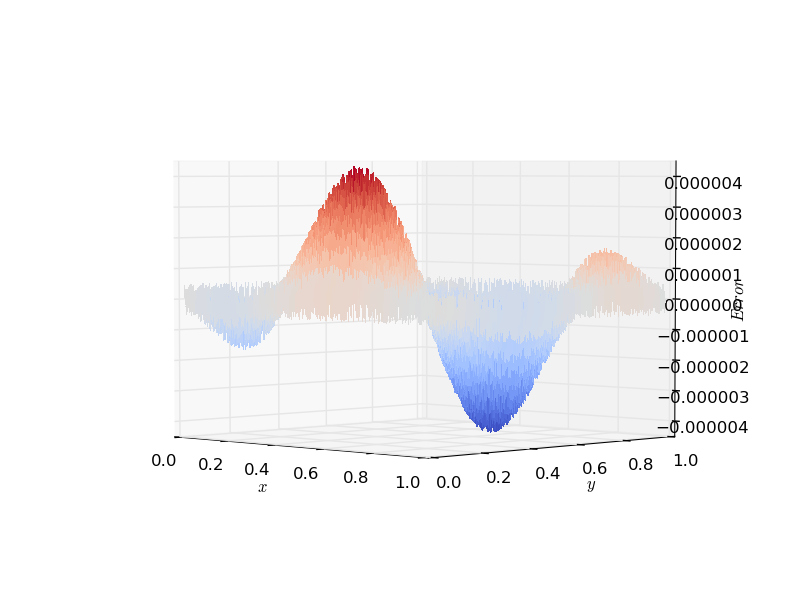
\includegraphics[width=1.0\linewidth]{images/example4_1000}
  \caption{$N = 1000 \quad (h = 0.001)$}
\end{subfigure}
\caption{Error ($u_{analytic} - u_{numerical}$) for decreasing $h = dx = dy$. The error gets smaller as we go from 200 to 1000 grid points (see Error axis range). }
\label{fig:example4.2}
\end{figure}

\chapter{Iterative Methods}
In this chapter, we will briefly describe the different iterative methods that have been implemented for the solution of the linear system of equations of the Poisson problem. After that, a convergence review will be given for the methods. A detailed analysis of the iterative methods is outside the scope of this report, but can be found in most numerical PDE books (e.g. \cite{leveque}).
\newline

The code for the iterative methods described in this chapter can be found in the \emph{iterative.c} source file. The desired iterative method can be chosen in \emph{main.c}, where it is passed as function pointer to the Poisson solver function.

\section{Jacobi Method}
The Jacobi method is the simplest iterative method that we will examine, and also the least efficient, as it has the slowest convergence. However, it is useful, not only as an example, but as a smoother in multigrid methods \cite{leveque}.
\newline

The Poisson problem we are solving can be written as follows, assuming that $dx = dy = h$, from equation (1.3): 

\begin{equation}
u_{i,j} = \frac{1}{4} \left(  u_{i-1, j} + u_{i+1, j} + u_{i, j-1} + u_{i, j+1}  \right) - \frac{h^2}{4}f_{i,j}
\end{equation}

The Jacobi method can be described by the following algorithm:

\begin{equation}
u_{i,j}^{k+1} = \frac{1}{4} \left(  u_{i-1, j}^k + u_{i+1, j}^k + u_{i, j-1}^k + u_{i, j+1}^k  \right) - \frac{h^2}{4}f_{i,j}
\end{equation}

where $u^{k}$ is the \emph{current} state of the solution, while $u^{k+1}$ is the new estimation. It is obvious that this method requires more memory, as the previous estimation of the solution has to be stored.
\newline

Alternatively, if we do not assume that $dx = dy$, as in equation (1.2), we write the Poisson problem as follows:

\begin{equation}
\begin{split}
u_{i,j} \quad = & \quad \frac{1}{2(dx^2 + dy^2)} \left(  (u_{i-1, j} + u_{i+1, j})dy^2 + (u_{i, j-1} + u_{i, j+1})dx^2  \right)\\
 & - \frac{dx^2 dy^2}{2(dx^2+dy^2)}f_{i,j}
\end{split}
\end{equation}

and the Jacobi method is now 

\begin{equation}
\begin{split}
u_{i,j}^{k+1} \quad = & \quad \frac{1}{2(dx^2 + dy^2)} \left(  (u_{i-1, j}^k + u_{i+1, j}^k)dy^2 + (u_{i, j-1}^k + u_{i, j+1}^k)dx^2  \right) \\
& - \frac{dx^2 dy^2}{2(dx^2+dy^2)}f_{i,j}
\end{split}
\end{equation}

\section{Gauss - Seidel Method}
The Gauss-Seidel method is a variation of the Jacobi method; it improves the solution by using the already calculated values for the new estimation. This simply translates to the following algorithm:

\begin{equation}
u_{i,j}^{k+1} = \frac{1}{4} \left(  u_{i-1, j}^{k+1} + u_{i+1, j}^k + u_{i, j-1}^{k+1} + u_{i, j+1}^k  \right) - \frac{h^2}{4}f_{i,j}
\end{equation}

or, keeping $dx \neq dy$:

\begin{equation}
\begin{split}
u_{i,j}^{k+1} \quad = & \quad \frac{1}{2(dx^2 + dy^2)} \left(  (u_{i-1, j}^{k+1} + u_{i+1, j}^k)dy^2 + (u_{i, j-1}^{k+1} + u_{i, j+1}^k)dx^2  \right) \\
 & - \frac{dx^2 dy^2}{2(dx^2+dy^2)}f_{i,j}
\end{split}
\end{equation}

The Gauss-Seidel method converges roughly twice as fast as the Jacobi method, and it does not require additional memory. However, it is less straightforward to parallelize (but can be parallelized using a red-black scheme \cite{karniadakis}).

\section{Successive Overrelaxation}
Successive overrelaxation (SOR) is an improvement on the Gauss-Seidel method, using an additional scalar parameter $\omega$, which is essentially moves the solution farther than Gauss-Seidel if $\omega > 1$ (and nearer if $\omega < 1$). SOR can be described by the following algorithm:

\begin{equation}
u_{i,j}^{k+1} = \frac{\omega}{2} \left(  u_{i-1, j}^{k+1} + u_{i+1, j}^k + u_{i, j-1}^{k+1} + u_{i, j+1}^k  \right) - \frac{h^2}{4}f_{i,j}
\end{equation}

and, in case that $dx \neq dy$:

\begin{equation}
\begin{split}
u_{i,j}^{k+1} \quad = & \quad \omega \left[ \frac{1}{2(dx^2 + dy^2)} 
\left(  (u_{i-1, j}^{k+1} + u_{i+1, j}^k)dy^2 + (u_{i, j-1}^{k+1} + u_{i, j+1}^k)dx^2  \right) \right.\\
& \left. - \frac{dx^2 dy^2}{2(dx^2+dy^2)}f_{i,j} \right] + (1 - \omega) u_{i,j}^k
\end{split}
\end{equation}

It should be mentioned that SOR is unstable for $\omega > 2$, while for $\omega = 1$ it is equivalent to the Gauss-Seidel method. Regarding the optimal choice for $\omega$, in general it depends on the problem (and may be hard to find). However, for the Poisson problem it can be shown that $\omega_{opt} \simeq 2 - 2 \pi h$ (\cite{leveque}, par. 4.2.2).

\section{Residual Checking}
Before commenting on the convergence of the previous methods, it will be useful to show the method followed in order to validate our iterative solution. The method followed is the well-known \emph{residual checking} method. This involves calculating the estimated solution between a fixed number of steps checking if the residual is smaller than a predetermined tolerance.
\newline

If $\bm{A}$ is the equation matrix and $\bm{u}$ is the estimated solution after a number of iterations, then

\begin{equation}
\bm{A} \bm{u} = \bm{f}_{est}
\end{equation}

But since we already know the right-hand values of our equations, we can quantify the correctness of our estimation by measuring how much our estimation differs from the actual right-hand side, by calculating the \emph{residual}:

\begin{equation}
r = \bm{A} \bm{u} - \bm{f}_{est}
\end{equation}

and stopping when it becomes smaller than some value that we set:

\begin{equation}
\sqrt{\sum_{i,j}r_{i,j}^2} < tolerance
\end{equation}

This procedure is carried out by the \emph{residual} function in \emph{src/poisson.c}.

\section{Convergence Comparison}
In this section we will show a brief comparison of the three iterative methods described in the revious sections. For this comparison, the Poisson problem shown in section (3.3) was solved, using $201 \times 201$ grid points.
\newline

To produce the following results, the program was altered slightly in order to output the residual in every iteration. Checking for the residual in every iteration is probably not worth the effort in general, but it is useful in order to evaluate the convergence of the three iterative methods.
\newline

We have set the maximum number of iterations to 1000 and the tolerance to zero; in this way, we can see the convergence of all three methods for 1000 iterations. Results are shown below using semi-log axes:
\newline

\begin{figure}[h!]
\centering
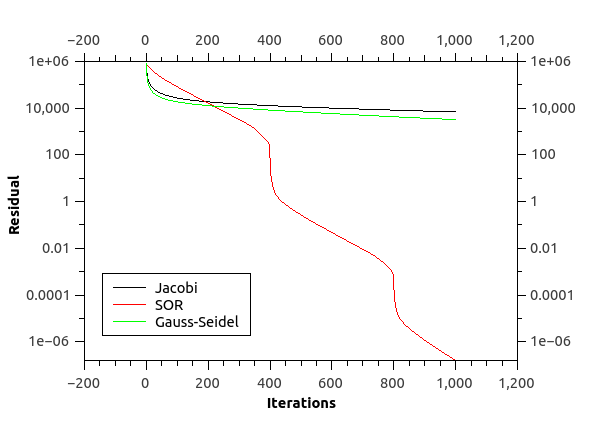
\includegraphics[width=0.75\linewidth]{images/residual}
\caption{Residual versus number of iterations, for 3 different iterative methods (Jacobi, Gauss-Seidel, SOR). Problem size: $201 \times 201$}
\label{fig:residual}
\end{figure}

We see that SOR is by far the most effective method. However, we should keep in mind that we are using the optimal $\omega$ value for SOR, which is known for this problem. Gauss-Seidel converges roughly twice as fast compared to Jacobi, something that is well known in general. Further analysis regarding the convergence of the iterative methods is outside the scope of this report, but can be found in \cite{leveque}, \cite{karniadakis}.

\chapter{Parallel Poisson Solver}
In this chapter, we will briefly show the parallel implementation of the Poisson solver in 2D, using OpenMP threads. A good review of OpenMP can be found in \cite{usingopenmp}. In this report, we will simply show the parallel implementation of the iterative solvers, along with their performance.

It should be mentioned that the code is maintained with the OpenMP directives, which can just be omitted if serial execution is desired. Also, for the Jacobi method, a number of OpenMP optimizations have been made, which are described in the next section; the uploaded code only features the optimized version. All other methods have their corresponding OpenMP parallel functions, starting with "redBlack" (from the red-black partitioning scheme, explained in section 5.2). To run in parallel, the user should choose the desired parallel function and compile.

OpenMP code can run as usual. First, we set the desired number of threads, for example for 4 threads we type:

\begin{lstlisting}
export OMP_NUM_THREADS=4
\end{lstlisting}

It is recommended, for systems using hyperthreading, to tie the threads to specific cores, using the command below (for this example using 4 threads):

\begin{lstlisting}
export GOMP_CPU_AFFINITY="0 1 2 3"
\end{lstlisting}

This ties the threads to the corresponding cores, ensuring that two different threads will not be assigned to a single hyperthreading core.

\section{Parallel Jacobi}
An initial parallelization of the Jacobi algorithm is very straightforward, and requires no further work. The OpenMP parallel version of the Jacobi method is shown below:

\begin{lstlisting}
#pragma omp parallel for schedule(static)\
                         shared(u, u_old, f)\
                         private(i,j)\
                         firstprivate(nX, nY, dx, dy)\
                         default(none)
for(i=1;i<nX-1;i++) {
  for(j=1;j<nY-1;j++) {
     u[i][j] = ((dy*dy)*(u_old[i-1][j] + u_old[i+1][j]) + 
               (dx*dx)*(u_old[i][j-1] + u_old[i][j+1]) - 
               (dx*dx)*(dy*dy)*f[i][j])/(2.0*((dx*dx) + (dy*dy)));
  }
}
\end{lstlisting}

Arrays are declared as \emph{shared} and no additional synchronization is required, since each thread only reads from and writes to its own part of the arrays. Array boundaries \emph{(nX, nY)} and values for \emph{(dx, dy)} are declared as \emph{firstprivate}, so that each thread has its own copy of these, with the correct initialized values. Finally, a static schedule is chosen with no chunksize specified. This results in the workload being equally distributed to the threads, in chunks equal to threads in number (for example, if we use 4 threads, the arrays will be divided into 4 parts).
\newline

We also parallelize the residual check in \emph{poisson.c}, in the following way:

\begin{lstlisting}
#pragma omp parallel for schedule(static)\
                         shared(u, rhs)\ 
                         private(i, j, Ax_r)\
                         firstprivate(nX, nY, dx, dy)\
                         reduction(+:res)\
                         default(none)
for (i=1; i<nX-1; i++) {
  for (j=1; j<nY-1; j++) {    
    Ax_r = ( 1.0/(dx*dx)*(u[i-1][j]-2.0*u[i][j]+u[i+1][j]) +
            1.0/(dy*dy)*(u[i][j-1]-2.0*u[i][j]+u[i][j+1]) -
            rhs[i][j] );
    res += Ax_r*Ax_r;
  }
}
\end{lstlisting}

The residual parallelization also takes place for the other iterative methods examined in the next sections. Apart from that, for the Jacobi method, we also parallelize the \emph{copyArray2D} function in \emph{iterative.c}. Without parallelizing the copy function, we end up in worse performance, due to poor cache memory distribution among threads.
\newline

Below we can see performance results for the OpenMP Jacobi method, for two different problem sizes.

\begin{figure}[h!]
\centering
\begin{subfigure}{0.45\textwidth}
  \centering
  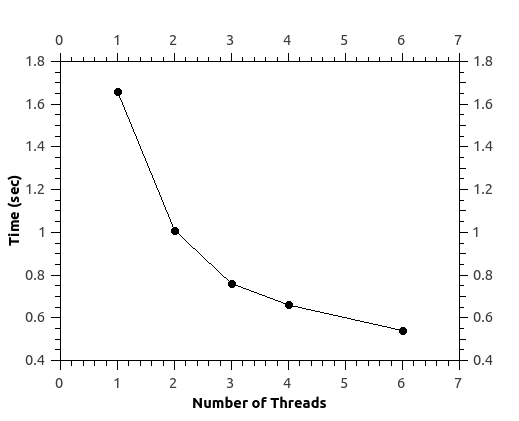
\includegraphics[width=1.0\linewidth]{images/jacobi_time_101}
  \caption{$Time$}
\end{subfigure}
\begin{subfigure}{0.45\textwidth}
  \centering
  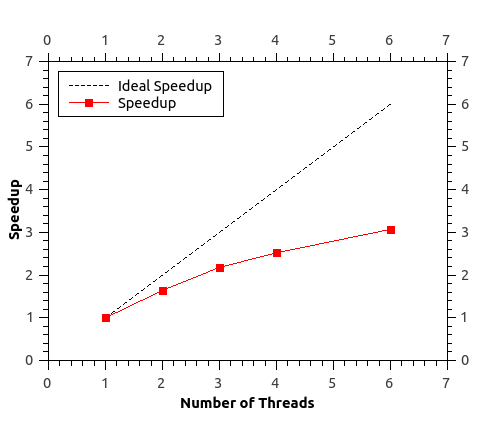
\includegraphics[width=1.0\linewidth]{images/jacobi_speedup_101}
  \caption{$Speedup$}
\end{subfigure}
\caption{Execution time and speedup for the OpenMP Jacobi implementation (problem size: $101 \times 101$) }
\label{fig:example5.1}
\end{figure}

\begin{figure}[th!]
\centering
\begin{subfigure}{0.45\textwidth}
  \centering
  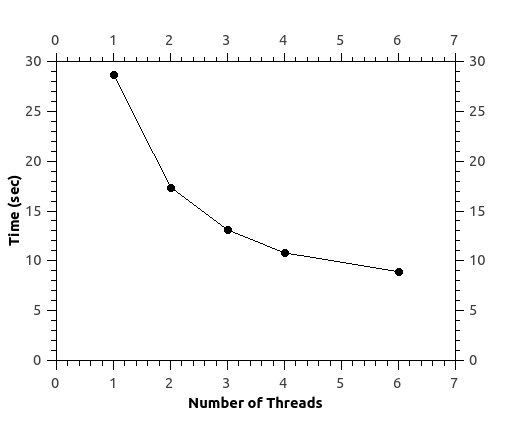
\includegraphics[width=1.0\linewidth]{images/jacobi_time_201}
  \caption{$Time$}
\end{subfigure}
\begin{subfigure}{0.45\textwidth}
  \centering
  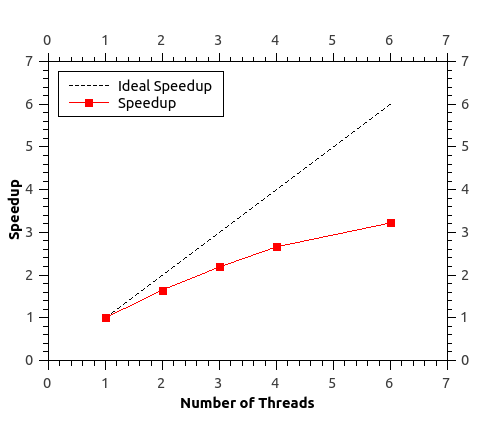
\includegraphics[width=1.0\linewidth]{images/jacobi_speedup_201}
  \caption{$Speedup$}
\end{subfigure}
\caption{Execution time and speedup for the OpenMP Jacobi implementation (problem size: $201 \times 201$) }
\label{fig:example5.2}
\end{figure}

\newpage

\subsection{An OpenMP Performance Optimization}
We notice that performance is worse than ideal for the initial Jacobi OpenMP implementation, something that may be attributed to the additional parallel regions by the \emph{copyArray2D} function, and also by another important factor: the initialization of the "u\_ old" arrays in memory ("\emph{array2D\_ contiguous}" function), in each Jacobi iteration. In the above experiments, arrays were initialized serially. This, however, leads to poor cache memory utilization; if all threads took part in the initialization, then they would have the memory in their cache for the subsequent iterations. Also, as NUMA architectures are prevalent, it is possible that memory is placed in the NUMA region where it is initialized, leading to cluttered communication for threads, reading and writing to NUMA regions further than optimal.
\newline

To improve performance and bypass the obstacles above, we can simply do two things: first, join the copy and Jacobi iterations into one parallel region, using two separate OpenMP worksharing directives, one for each loop. In this way, we end up with half as many parallel regions opened and closed in each iteration, hopefully removing much of the overhead.
\newline

Second, we can do the array initialization to zero in parallel, in the \emph{array2D\_ contiguous}, in \emph{memory.c}. In this way, each thread will initialize the part of the array it will work on in the Jacobi iterations, both keeping that memory in cache and also in its corresponding NUMA region. It is, of course, important to keep the same worksharing schedule in all parallel regions, for obvious reasons; otherwise, each thread would possibly initialize another thread's array elements, negating the cache memory and NUMA advantages mentioned.
\newline

Doing the above, we repeat the performance tests and summarize the results in the following figures, showing both initial and optimized OpenMP versions (and also ideal/linear scaling).

\begin{figure}[h!]
\centering
\begin{subfigure}{0.45\textwidth}
  \centering
  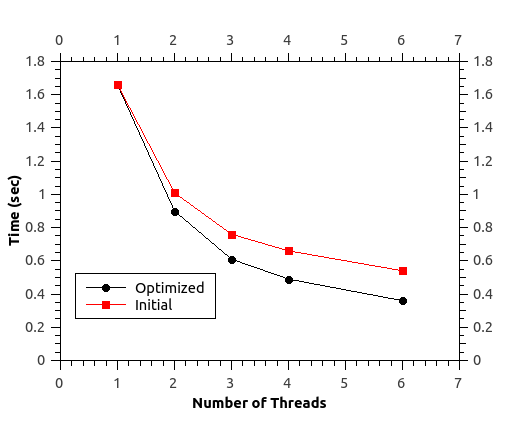
\includegraphics[width=1.0\linewidth]{images/jacobi_time_101_opt}
  \caption{$Time$}
\end{subfigure}
\begin{subfigure}{0.45\textwidth}
  \centering
  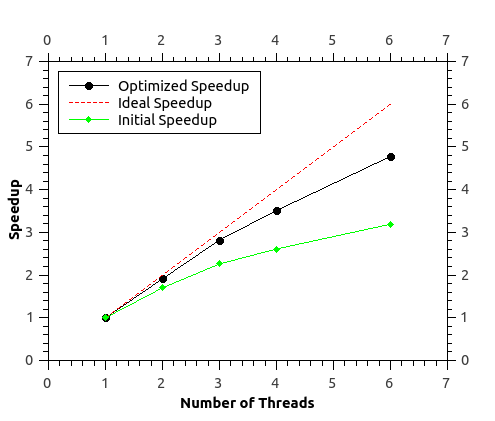
\includegraphics[width=1.0\linewidth]{images/jacobi_speedup_101_opt}
  \caption{$Speedup$}
\end{subfigure}
\caption{Execution time and speedup for the optimized OpenMP Jacobi implementation (problem size: $101 \times 101$). The initial performance is also shown, for comparison. }
\label{fig:example5.3}
\end{figure}

\newpage

\begin{figure}[th!]
\centering
\begin{subfigure}{0.45\textwidth}
  \centering
  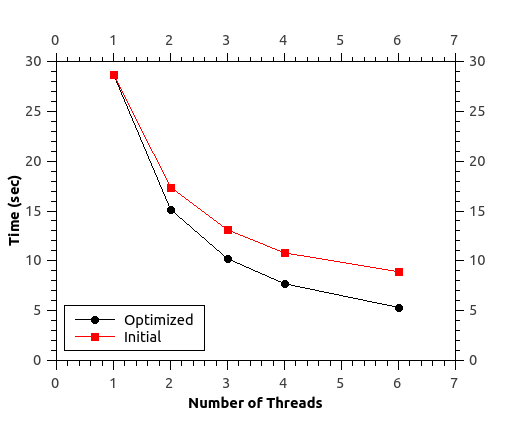
\includegraphics[width=1.0\linewidth]{images/jacobi_time_201_opt}
  \caption{$Time$}
\end{subfigure}
\begin{subfigure}{0.45\textwidth}
  \centering
  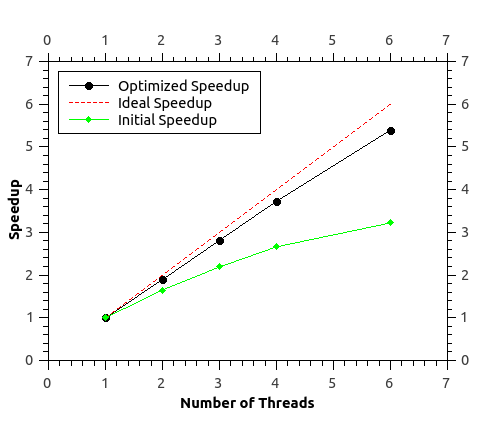
\includegraphics[width=1.0\linewidth]{images/jacobi_speedup_201_opt}
  \caption{$Speedup$}
\end{subfigure}
\caption{Execution time and speedup for the optimized OpenMP Jacobi implementation (problem size: $201 \times 201$). The initial speedup is also shown, for comparison. }
\label{fig:example5.4}
\end{figure}

It is obvious that performance has clearly improved and is actually near the ideal performance, for the larger problem size. This was a good example of OpenMP optimization. Although that the Jacobi method was trivial to parallelize, it required a number of alterations to achieve good performance. It should be mentioned that the code is maintained \emph{with} the optimizations described here.

\section{Parallel Gauss-Seidel}
The Gauss-Seidel is less trivial to parallelize than Jacobi. In general, a \emph{red-black} (or \emph{checkerboard}) approach is followed, in which we update the grid elements in two separate groups ("red" and "black"), as in a checkerboard. We will not describe the method further in this report, but a good description can be found at \cite{karniadakis}.
\newline

The parallelized Gauss-Seidel algorithm can be found in the function \emph{redBlackGaussSeidelIteration2D}, in \emph{iterative.c}. Below we can see performance results for the Gauss-Seidel method in parallel, following the red-black scheme.

\begin{figure}[th!]
\centering
\begin{subfigure}{0.45\textwidth}
  \centering
  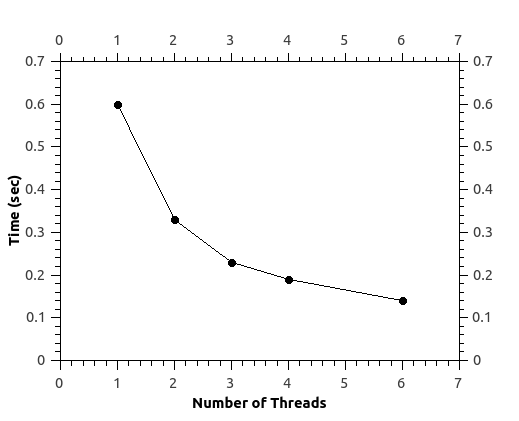
\includegraphics[width=1.0\linewidth]{images/gauss_time_101}
  \caption{$Time$}
\end{subfigure}
\begin{subfigure}{0.45\textwidth}
  \centering
  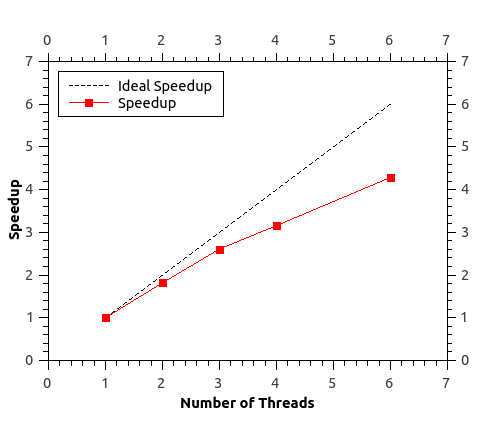
\includegraphics[width=1.0\linewidth]{images/gauss_speedup_101}
  \caption{$Speedup$}
\end{subfigure}
\caption{Execution time and speedup for the OpenMP Gauss-Seidel implementation (problem size: $101 \times 101$). }
\label{fig:example5.5}
\end{figure}

\begin{figure}[th!]
\centering
\begin{subfigure}{0.45\textwidth}
  \centering
  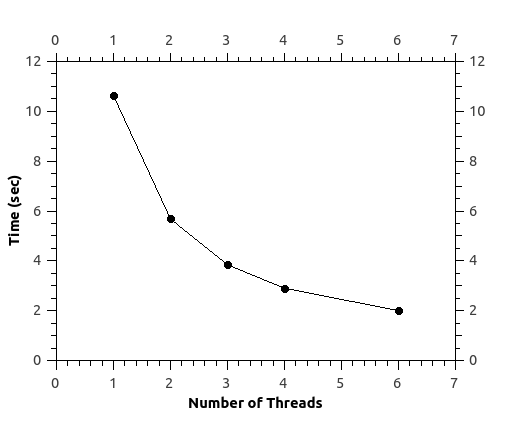
\includegraphics[width=1.0\linewidth]{images/gauss_time_201}
  \caption{$Time$}
\end{subfigure}
\begin{subfigure}{0.45\textwidth}
  \centering
  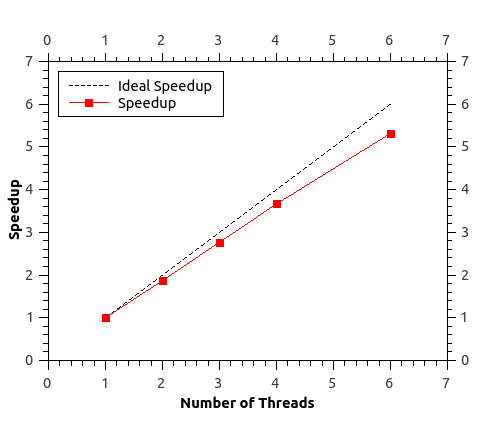
\includegraphics[width=1.0\linewidth]{images/gauss_speedup_201}
  \caption{$Speedup$}
\end{subfigure}
\caption{Execution time and speedup for the OpenMP Gauss-Seidel implementation (problem size: $201 \times 201$). }
\label{fig:example5.6}
\end{figure}

\newpage

We see that OpenMP performance for the Gauss-Seidel method is decent, especially for the larger problem size. Regarding the smaller problem size, the execution times show that the method requires few iterations to converge and, along with the small grid, this means that the workload is not so heavy to fully utilize all threads, for higher thread counts. Still, the OpenMP code manages to achieve speedup for all cases. We expect even larger problem sizes to scale even better, however such tests were not carried out for this report, in order to save core hours.

\section{Parallel Successive Overrelaxation}
Parallelizing the SOR method is very similar to parallelizing the Gauss-Seidel method. Again, we follow a \emph{red-black} scheme and the SOR OpenMP function is named \emph{"redBlackSORIteration2D"}, in \emph{iteration.c}, where the OpenMP code can be found. 
\newline

Due to the fact that SOR converges very fast for this Poisson problem, it is sensible (and possible) to show scaling tests for larger grids with this method. Performance results are shown in the following figures.

\begin{figure}[th!]
\centering
\begin{subfigure}{0.45\textwidth}
  \centering
  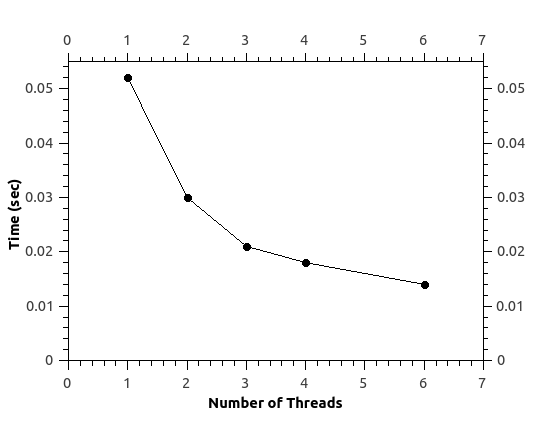
\includegraphics[width=1.0\linewidth]{images/sor_time_101}
  \caption{$Time$}
\end{subfigure}
\begin{subfigure}{0.45\textwidth}
  \centering
  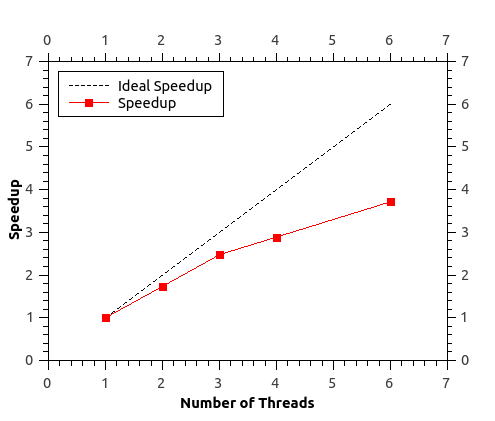
\includegraphics[width=1.0\linewidth]{images/sor_speedup_101}
  \caption{$Speedup$}
\end{subfigure}
\caption{Execution time and speedup for the OpenMP SOR implementation (problem size: $101 \times 101$). }
\label{fig:example5.7}
\end{figure}

\begin{figure}[th!]
\centering
\begin{subfigure}{0.45\textwidth}
  \centering
  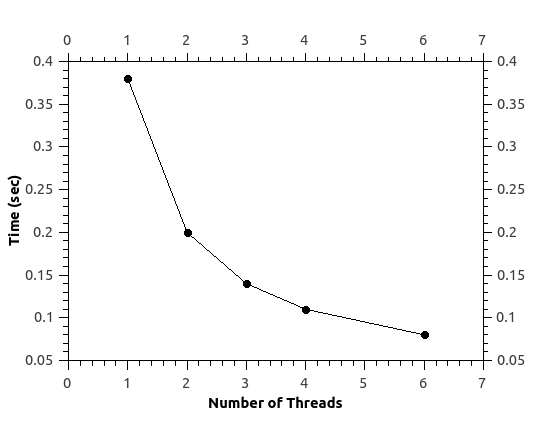
\includegraphics[width=1.0\linewidth]{images/sor_time_201}
  \caption{$Time$}
\end{subfigure}
\begin{subfigure}{0.45\textwidth}
  \centering
  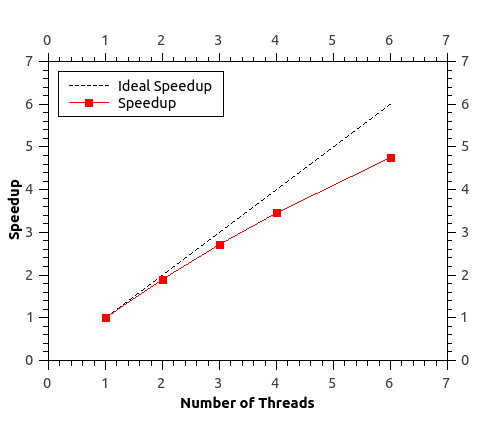
\includegraphics[width=1.0\linewidth]{images/sor_speedup_201}
  \caption{$Speedup$}
\end{subfigure}
\caption{Execution time and speedup for the OpenMP SOR implementation (problem size: $201 \times 201$). }
\label{fig:example5.7}
\end{figure}

\begin{figure}[th!]
\centering
\begin{subfigure}{0.45\textwidth}
  \centering
  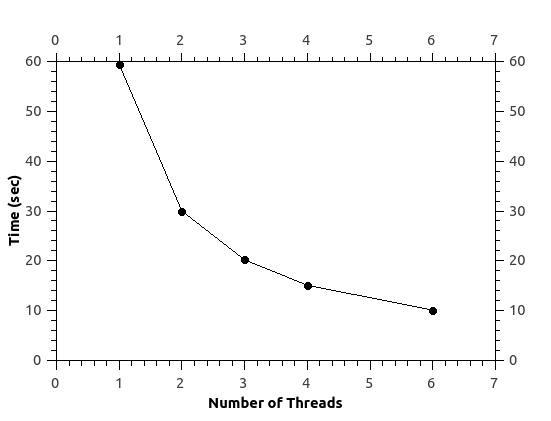
\includegraphics[width=1.0\linewidth]{images/sor_time_1001}
  \caption{$Time$}
\end{subfigure}
\begin{subfigure}{0.45\textwidth}
  \centering
  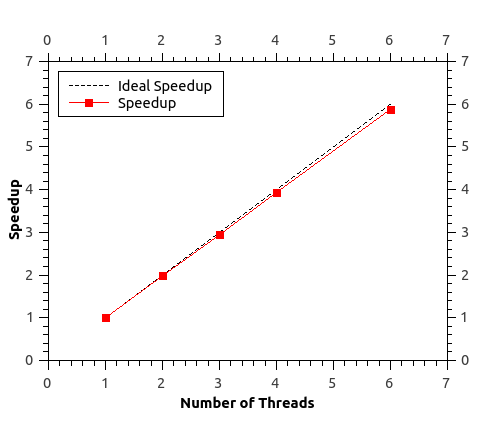
\includegraphics[width=1.0\linewidth]{images/sor_speedup_1001}
  \caption{$Speedup$}
\end{subfigure}
\caption{Execution time and speedup for the OpenMP SOR implementation (problem size: $1001 \times 1001$). }
\label{fig:example5.8}
\end{figure}

\newpage

Again, sizes $101 \times 101$ and $201 \times 201$ follow a similar trend, achieving better scaling as the grid size increases. It is worth noticing how much faster the SOR method converges, taking 5\% of a second with a single thread for the smaller size.
\newline

However, the larger size of $1001 \times 1001$ is where the OpenMP parallel implementation truly shines, achieving practically ideal speedup, as shown in figure 5.9.b. This leads us to expect similar scaling behavior in the other iterative methods (although with much larger execution times).
\newline




\begin{thebibliography}{1}

  \bibitem{leveque} Randall J. LeVeque {\em Finite Difference Methods for Ordinary and Partial Differential Equations.}  2007.

  \bibitem{karniadakis} George Em. Karniadakis, Robert M. Kirby {\em Parallel Scientific Computing in C++ and MPI.} 2003 

  \bibitem{usingopenmp} Barbara Chapman, Gabrielle Jost, Ruud Van Der Pas {\em Using OpenMP.} 2008.

  \end{thebibliography}

\end{document}